\documentclass[a4paper,12pt]{article}
\usepackage{tikz, pgfplots}
\pgfplotsset{compat=newest}
\usepackage{xcolor}
\usepackage[left=2cm,right=2cm,top=2cm,bottom=2cm]{geometry}
\usepackage{lipsum} % For sample text
\usepackage{ebgaramond}
\fontsize{14}{14}\selectfont % Increase the font size to 12pt

%\fontsize{\}{skip}
% Define Colors
\definecolor{myBrown}{RGB}{89, 40, 13}
\definecolor{pagetitlecolor}{RGB}{89, 40, 13}
\definecolor{customcolor}{RGB}{100,65,5}
\definecolor{pgfbackgroundcolor}{RGB}{245,225,185}
\definecolor{pgfnodecolor}{RGB}{55,40,30}


% Add tikz library for patterns
\usetikzlibrary{patterns}

% Custom section titles
\usepackage{titlesec}
\titleformat{\section}
{\normalfont\Large\bfseries\color{myBrown}}{\thesection}{1em}{}

% Increase paragraph spacing and indentation
%\setlength{\parskip}{1em}
%\setlength{\parindent}{1.5em}

\title{\color{pagetitlecolor}\textbf{Evolving Class Sizes at Galileo Galilei Elementary}}
\author{\textit{An Insightful Five-Year Overview}}
\date{}

\begin{document}


\maketitle
\thispagestyle{empty}

Galileo Galilei Elementary School has experienced a fluctuating journey with regard to class sizes over the past five years. Every year brought new successes and challenges, ranging from shifts in educational policies to variations in student enrollment.
\vspace{1em}

\begin{center}
    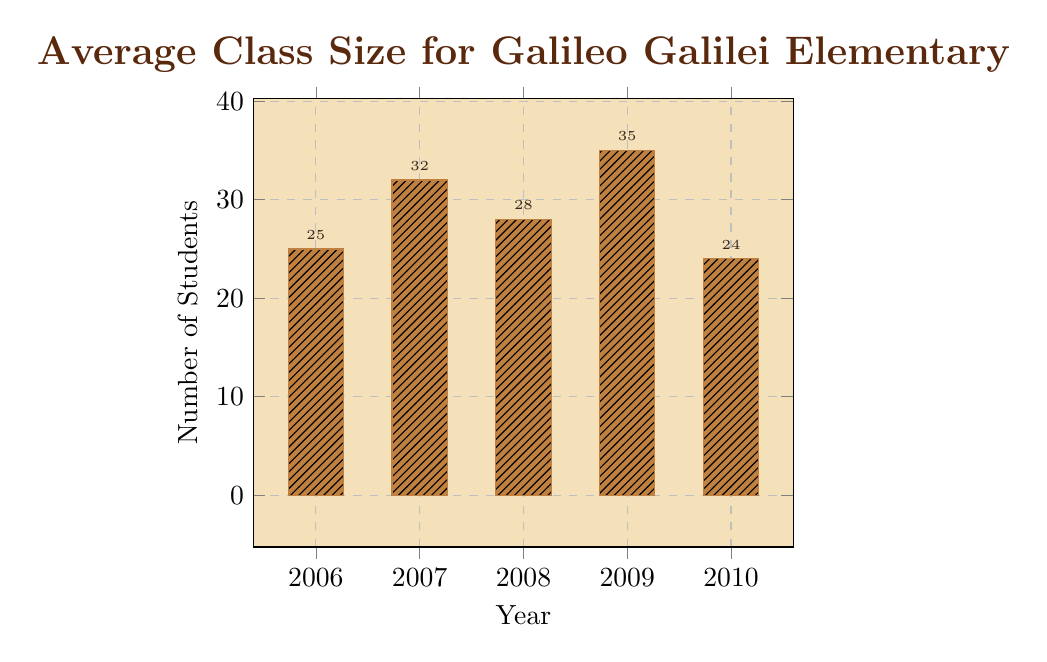
\begin{tikzpicture}
        \begin{axis}[
                ybar, % Bar graph
                bar width=20pt, % Width of the bars
                title={\color{myBrown}Average Class Size for Galileo Galilei Elementary}, % Main title
                title style={align=center, font=\Large\bfseries}, % Center the title if it wraps
                enlargelimits=0.15,
                ylabel={Number of Students}, % Label for the y-axis
                xlabel={Year}, % Label for the x-axis
                symbolic x coords={2006, 2007, 2008, 2009, 2010},
                xtick=data,
                nodes near coords, % Display data value near bars
                nodes near coords align={vertical},
                % apply color to noes near cords
                every node near coord/.append style={font=\tiny, color=pgfnodecolor},
                ymin=0, ymax=35, % Adjusted for better fit of the annotation
                xmajorgrids=true,
                ymajorgrids=true,
                grid style=dashed,
                axis background/.style={fill=pgfbackgroundcolor}, % Background color for the plot area
                ]
            
            \addplot +[
                postaction={
                    pattern=north east lines
                },
                fill=brown, % Softer brown color
                draw=brown,
                ] coordinates {(2006,25) (2007,32) (2008,28) (2009,35) (2010,24)};
            
        \end{axis}
    \end{tikzpicture}
\end{center}

These changes are shown in a simple, visual style in the graph above. 2009 is noticeable for having the largest average class size during a peak in the number of students enrolled in the school. During this time, deliberate changes were made in the curriculum and in teachers in order to preserve the standard of education.

As we step into the future, Galileo Galilei Elementary continues to adapt and evolve. The insights gained from the past five years are invaluable in shaping a responsive and dynamic educational environment for our young learners.

\end{document}
